\section{Resoconto delle attività di verifica}
In questa sezione vengono descritti ed analizzati gli esiti delle attività di verifica su tutti i documenti destinati alla consegna.

\subsection{Revisione dei requisiti}

\subsubsection{Analisi statica dei documenti}
I membri del gruppo \Gruppo{} hanno analizzato i documenti mediante la tecnica di walkthrough che ha portato all'individuazione di 
alcuni errori ortografici e grammaticali, grazie anche agli strumenti di controllo ortografico integrati negli editor per la produzione
della documentazione che il gruppo ha deciso di utilizzare.

\subsubsection{Esiti verifiche automatizzate}
Attualmente, l'unico valore che può essere calcolato per \glo{verificare} se la garanzia di qualità che il gruppo ritiene fornire è
soddisfatta, è data dall'Indice di Gulpease (MPC6).
%Per poter calcolare questo indice, viene utilizzato come strumento il "Calcolatore dell'Indice Gulpease" ospitato a \href{https://farfalla-project.org/readability_static/}{questo indirizzo}.
%Non vengono contati per l'indice di Gulpease il testo presente nelle seguenti parti o sezioni del documento:
%\begin{itemize}
  %  \item Indice;
  %  \item Registro delle modifiche;
  %  \item Riferimenti.
%\end{itemize}
Nella seguente tabella sono riportati i risultati degli indici di Gulpease ottenuti dai documenti per ogni periodo, successivamente ci sarà un grafico che riporterà l'andamento degli indici di Gulpease per ogni documento a seconda del periodo.

\paragraph{Legenda - Tabella Gulpease}
\begin{itemize}
	\item \textbf{Documento}: Nome del documento;
	\item \textbf{RR}: Periodo di revisione dei requisiti;
	\item  \textbf{Colore giallo}: Indica che il valore ottenuto è accettabile;
	\item  \textbf{Colore verde}: Indica che il valore ottenuto è ottimo. 
\end{itemize}

\paragraph{MPC6 - Indice di Gulpease}

\rowcolors{2}{grigetto}{white}
\renewcommand{\arraystretch}{1.5}
\begin{longtable}{C{4cm} C{1cm} C{1cm} C{1cm} C{1cm}}
\caption{Elenco degli indici di Gulpease }\\
\rowcolor{darkblue}
\textcolor{white}{\textbf{Documento}} & \textcolor{white}{\textbf{RR}} \\
\hline
\endhead
\AdRv{1.0.0} & \textcolor{verde}{\textbf{95}} \\
\PdPv{1.0.0} & \textcolor{verde}{\textbf{100}} \\
\PdQv{1.0.0} & \textcolor{verde}{\textbf{100}} \\

\NdPv{1.0.0} & \textcolor{giallo}{\textbf{75}} \\
\SdFv{1.0.0} & \textcolor{verde}{\textbf{94}} \\

\Glossariov{1.0.0} & \textcolor{giallo}{\textbf{67}} \\

Media verbali interni & \textcolor{verde}{\textbf{92}} \\
Media verbali esterni & \textcolor{giallo}{\textbf{65}} \\

\end{longtable}

%\begin{figure}[h]
%	\centering
%	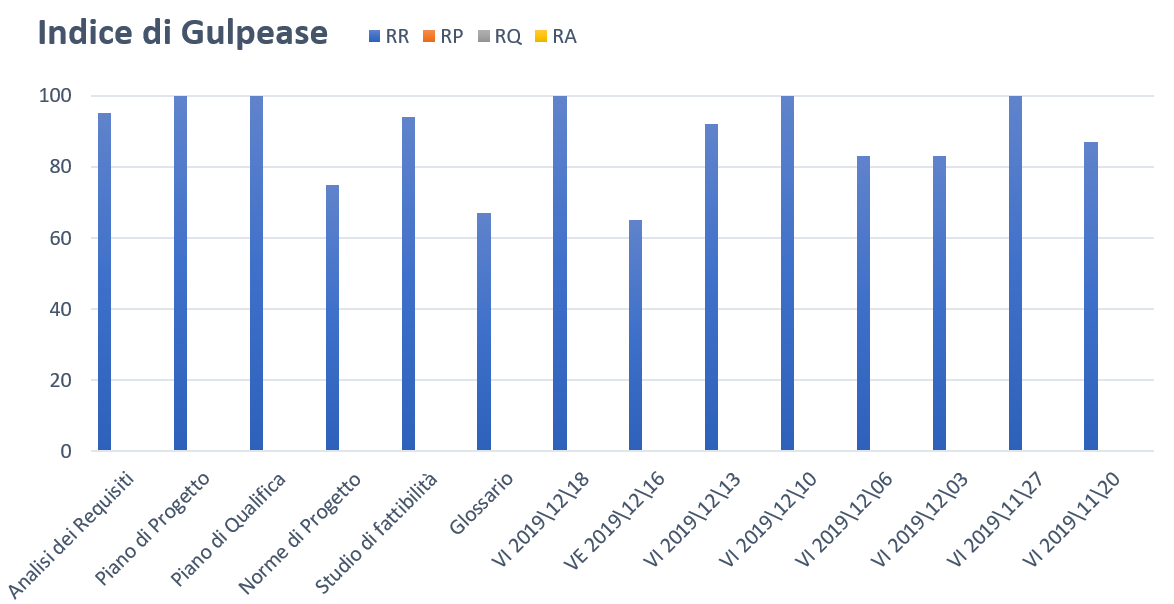
\includegraphics[scale=0.50]{Sezioni/Immagini/IG-Grafico.png}
%	\caption{Grafico andamento dell'Indice di Gulpease per ogni periodo e documento}
%\end{figure}
%}
\newpage
\pgfplotsset{width=17cm, height=10cm}
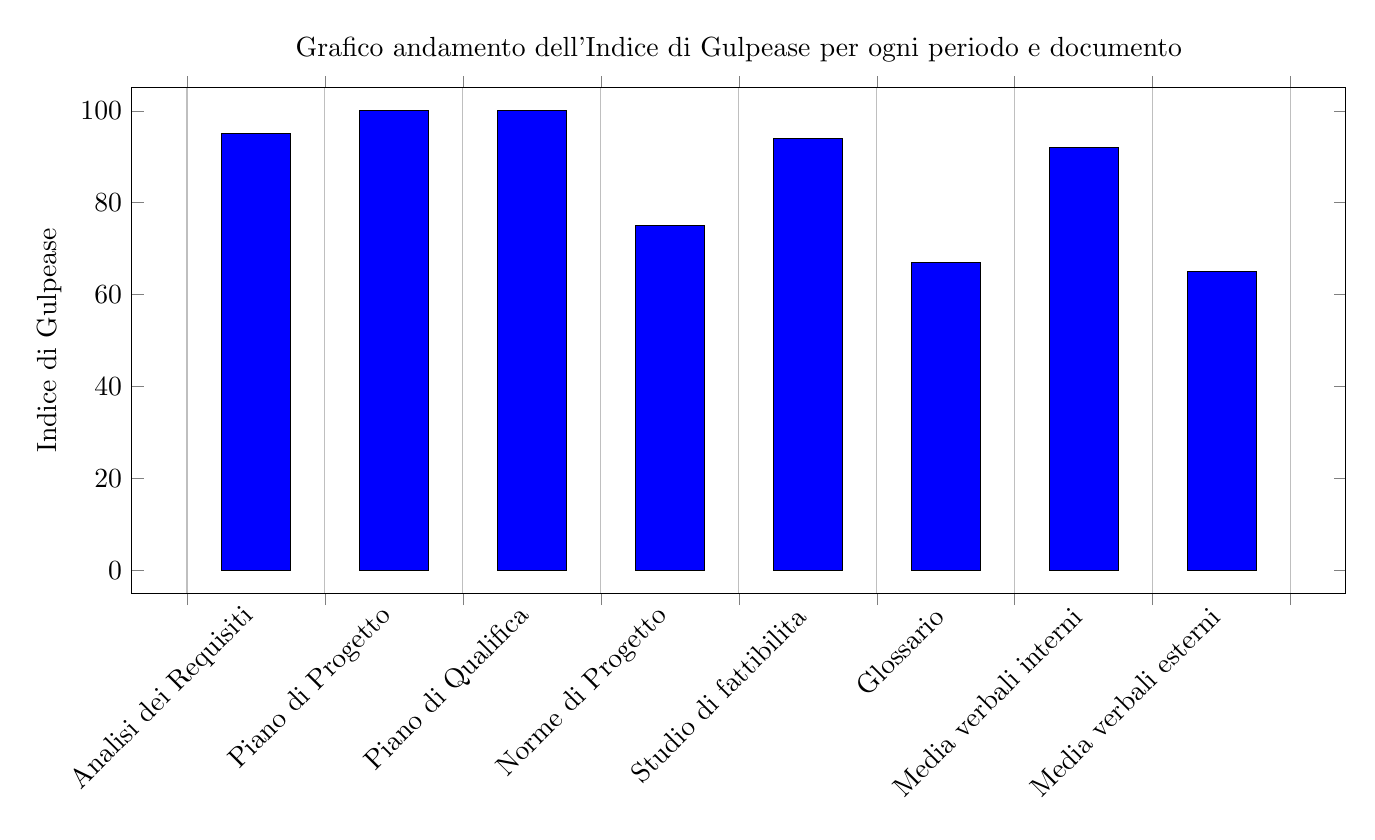
\begin{tikzpicture}

\begin{axis}[
title=Grafico andamento dell'Indice di Gulpease per ogni periodo e documento,
x tick label style={
/pgf/number format/1000 sep=},
ylabel=Indice di Gulpease,
enlargelimits=0.05,
legend style={at={(0.5,-0.4)},
anchor=north,legend columns=-1},
ybar interval=0.5,
symbolic x coords={Analisi dei Requisiti, Piano di Progetto, Piano di Qualifica, Norme di Progetto, Studio di fattibilita, Glossario,
Media verbali interni, Media verbali esterni, tmp},%lasciare tmp come ultima colonna per poter visualizzare tutte le colonne tranne tmp
x tick label style={rotate=45,anchor=east},
xtick=data
]
\addplot[fill=blue] coordinates
{(Analisi dei Requisiti, 95) (Piano di Progetto, 100) (Piano di Qualifica, 100) 
(Norme di Progetto, 75) (Studio di fattibilita, 94) (Glossario, 67)
(Media verbali interni, 92) (Media verbali esterni, 65) (tmp, 0)};

\end{axis}
\end{tikzpicture}


\subsection{Revisione di progettazione}
aaaa
\subsubsection{Analisi statica dei documenti}
aaaaa

\subsubsection{Esiti verifiche automatizzate}
aaaaa

\paragraph{MPC1 - Percentuale requisiti obbligatori soddisfatti} 

\pgfplotsset{width=17cm, height=8cm}
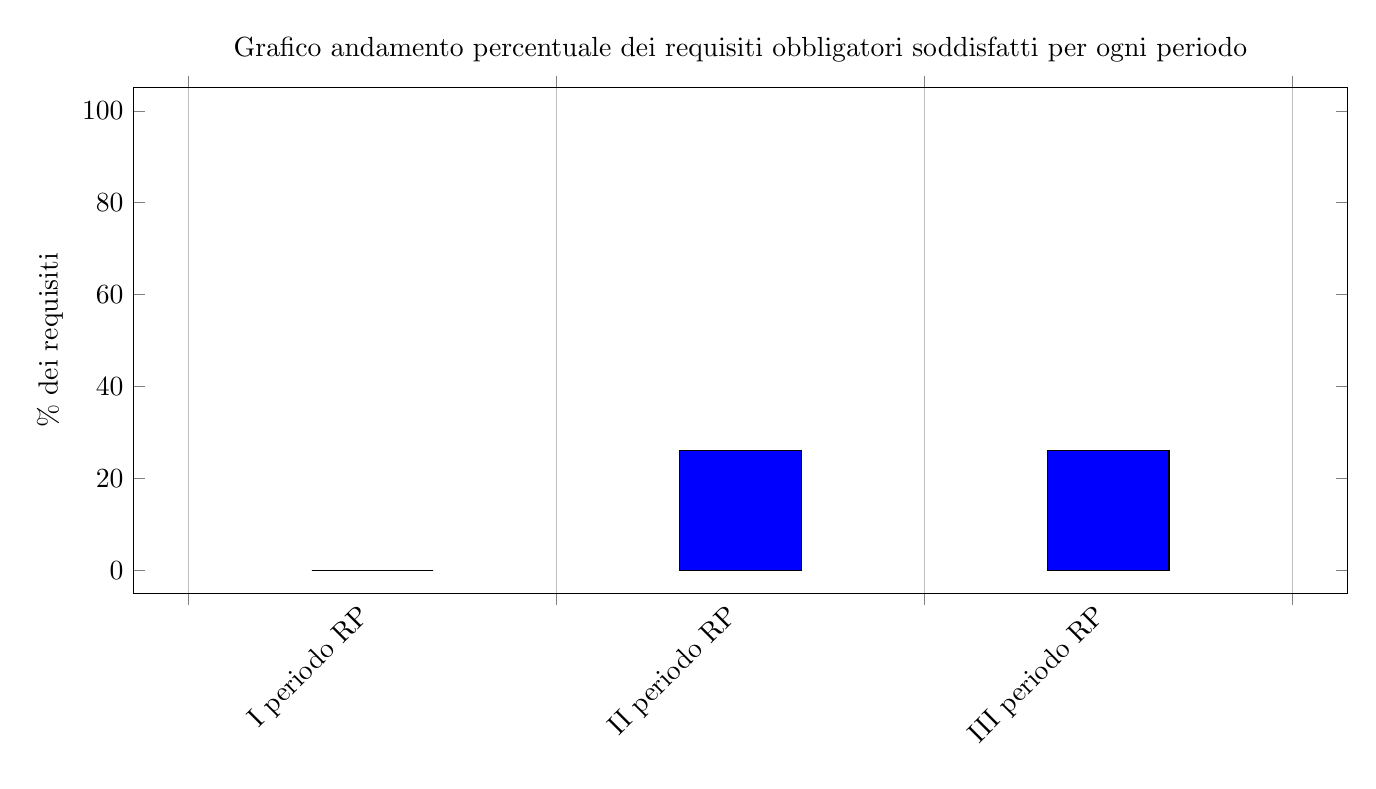
\begin{tikzpicture}

\begin{axis}[
title=Grafico andamento percentuale dei requisiti obbligatori soddisfatti per ogni periodo,
x tick label style={
	/pgf/number format/1000 sep=},
ylabel=\% dei requisiti,
enlargelimits=0.05,
legend style={at={(0.5,-0.4)},
	anchor=north,legend columns=-1},
ybar interval=0.33,
symbolic x coords={I periodo RP, II periodo RP, III periodo RP, tmp},%lasciare tmp come ultima colonna per poter visualizzare tutte le colonne tranne tmp
x tick label style={rotate=45,anchor=east},
xtick=data
]
\addplot[fill=blue] coordinates
{(I periodo RP, 0) (II periodo RP, 26) (III periodo RP, 26) (tmp, 100)};

\end{axis}
\end{tikzpicture}

\paragraph{MPC2 - Incapsulamento CBO}

\pgfplotsset{width=17cm, height=8cm}
\begin{tikzpicture}

\begin{axis}[
title=Grafico andamento incapsulamento CBO per ogni periodo,
x tick label style={
	/pgf/number format/1000 sep=},
ylabel=incapsulamento CBO,
enlargelimits=0.05,
legend style={at={(0.5,-0.4)},
	anchor=north,legend columns=-1},
ybar interval=0.33,
symbolic x coords={I periodo RP, II periodo RP, III periodo RP, tmp},%lasciare tmp come ultima colonna per poter visualizzare tutte le colonne tranne tmp
x tick label style={rotate=45,anchor=east},
xtick=data
]
\addplot[fill=blue] coordinates
{(I periodo RP, 0) (II periodo RP, 0) (III periodo RP, 0) (tmp, 100)};
\end{axis}
\end{tikzpicture}

\paragraph{MPC3 - Livello profondità gerarchia}

\pgfplotsset{width=17cm, height=8cm}
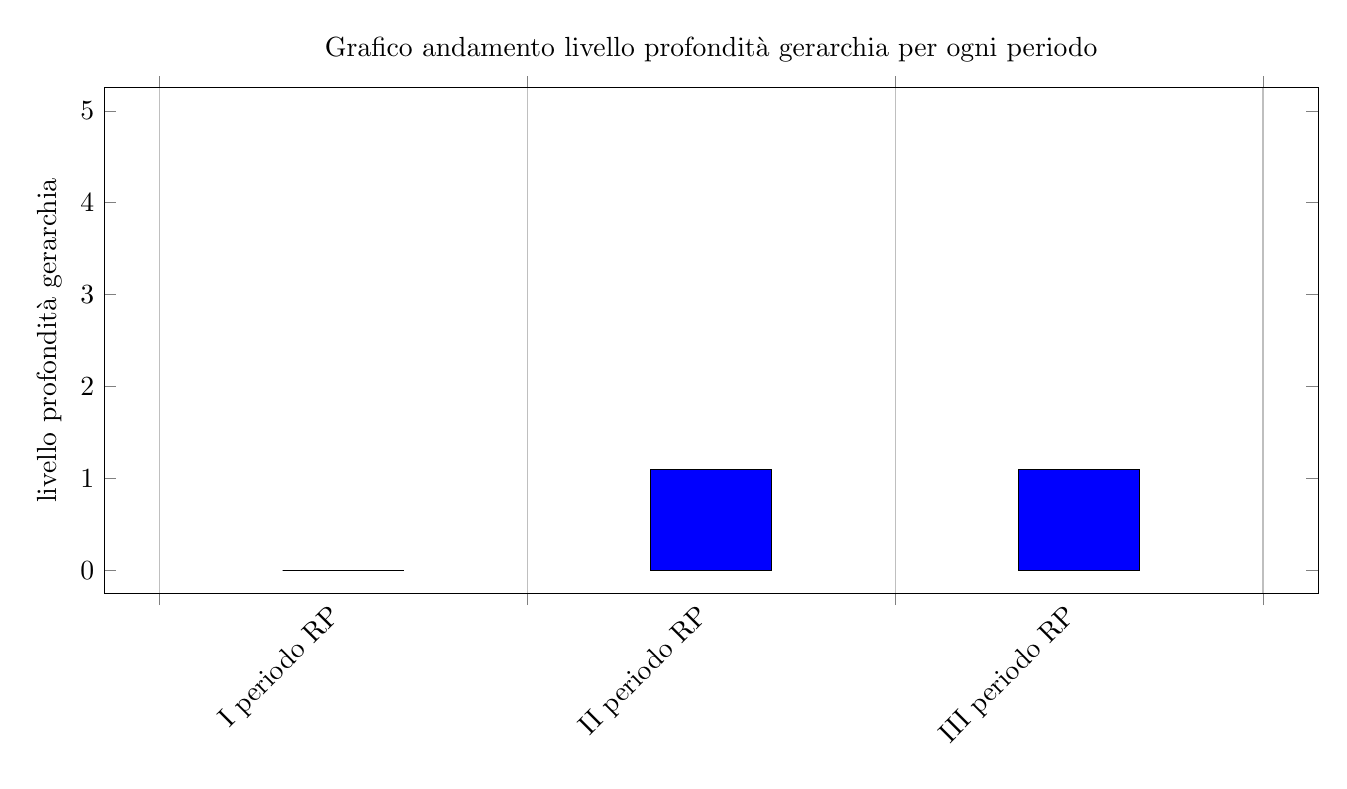
\begin{tikzpicture}

\begin{axis}[
title=Grafico andamento livello profondità gerarchia per ogni periodo,
x tick label style={
	/pgf/number format/1000 sep=},
ylabel=livello profondità gerarchia,
enlargelimits=0.05,
legend style={at={(0.5,-0.4)},
	anchor=north,legend columns=-1},
ybar interval=0.33,
symbolic x coords={I periodo RP, II periodo RP, III periodo RP, tmp},%lasciare tmp come ultima colonna per poter visualizzare tutte le colonne tranne tmp
x tick label style={rotate=45,anchor=east},
xtick=data
]
\addplot[fill=blue] coordinates
{(I periodo RP, 0) (II periodo RP, 1.1) (III periodo RP, 1.1) (tmp, 5)};

\end{axis}
\end{tikzpicture}

\paragraph{MPC4 - Numero di parametri per metodo}

\pgfplotsset{width=17cm, height=8cm}
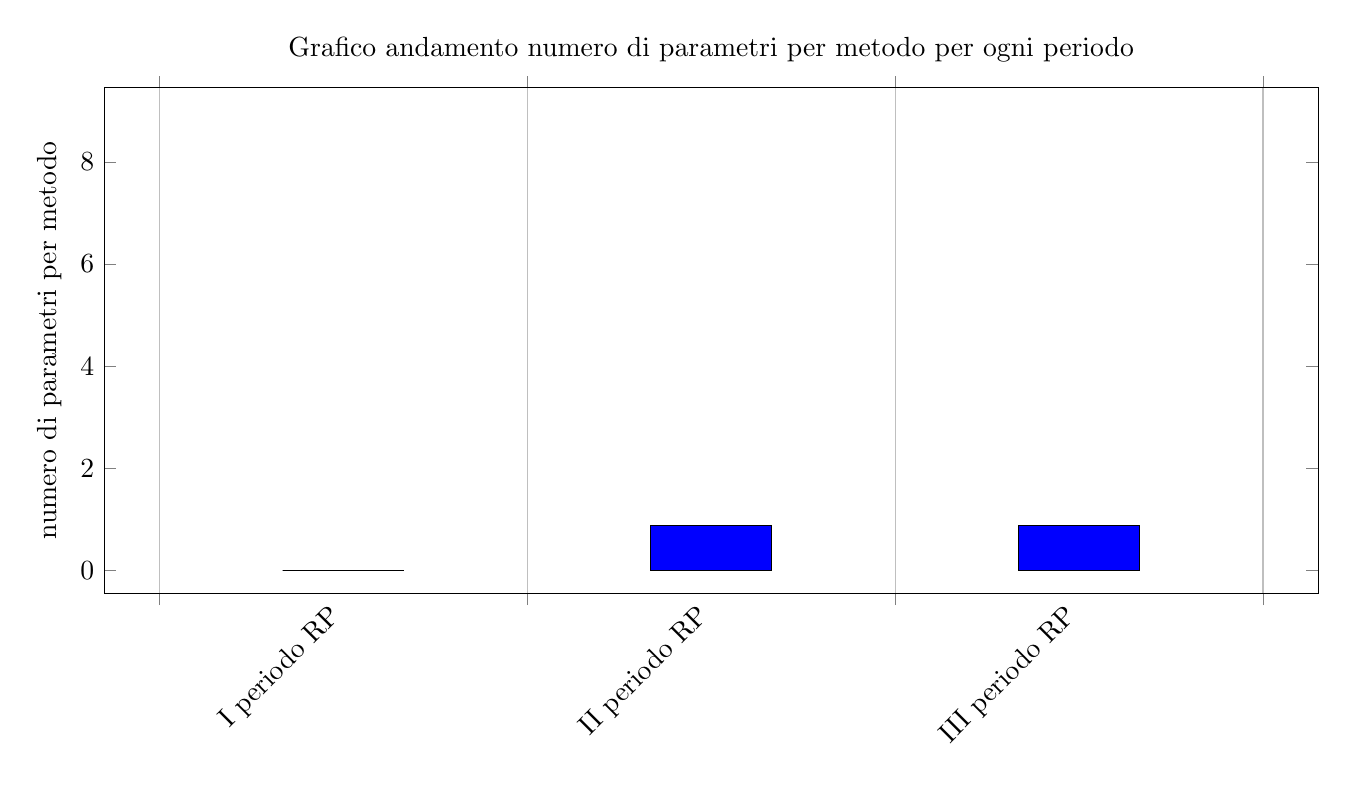
\begin{tikzpicture}

\begin{axis}[
title=Grafico andamento numero di parametri per metodo per ogni periodo,
x tick label style={
	/pgf/number format/1000 sep=},
ylabel=numero di parametri per metodo,
enlargelimits=0.05,
legend style={at={(0.5,-0.4)},
	anchor=north,legend columns=-1},
ybar interval=0.33,
symbolic x coords={I periodo RP, II periodo RP, III periodo RP, tmp},%lasciare tmp come ultima colonna per poter visualizzare tutte le colonne tranne tmp
x tick label style={rotate=45,anchor=east},
xtick=data
]
\addplot[fill=blue] coordinates
{(I periodo RP, 0) (II periodo RP, 0.87) (III periodo RP, 0.87) (tmp, 9)};

\end{axis}
\end{tikzpicture}

\paragraph{MPC5 - Linee di commento per linee di codice}
\pgfplotsset{width=17cm, height=8cm}
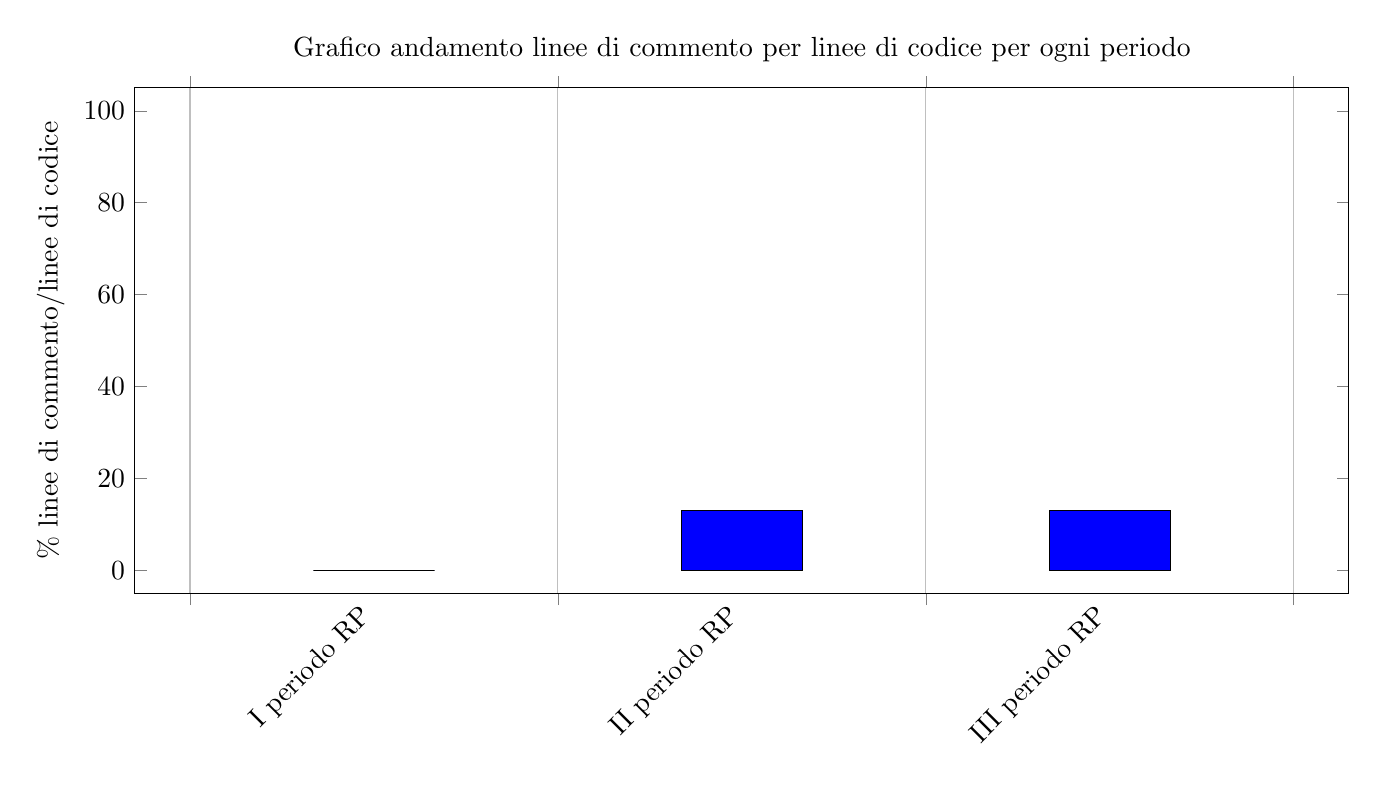
\begin{tikzpicture}

\begin{axis}[
title=Grafico andamento linee di commento per linee di codice per ogni periodo,
x tick label style={
	/pgf/number format/1000 sep=},
ylabel=\% linee di commento/linee di codice,
enlargelimits=0.05,
legend style={at={(0.5,-0.4)},
	anchor=north,legend columns=-1},
ybar interval=0.33,
symbolic x coords={I periodo RP, II periodo RP, III periodo RP, tmp},%lasciare tmp come ultima colonna per poter visualizzare tutte le colonne tranne tmp
x tick label style={rotate=45,anchor=east},
xtick=data
]
\addplot[fill=blue] coordinates
{(I periodo RP, 0) (II periodo RP, 13) (III periodo RP, 13) (tmp, 100)};

\end{axis}
\end{tikzpicture}


\paragraph{MPC6 - Indice di Gulpease}

\rowcolors{2}{grigetto}{white}
\renewcommand{\arraystretch}{1.5}
\begin{longtable}{C{4cm} C{2cm} C{2cm} C{2cm} C{2cm}}
	\caption{Elenco degli indici di Gulpease }\\
	\rowcolor{darkblue}
	\textcolor{white}{\textbf{Documento}} & \textcolor{white}{\textbf{I periodo RP}} &
	\textcolor{white}{\textbf{II periodo RP}} & \textcolor{white}{\textbf{III periodo RP}} \\
	\hline
	\endhead
	\AdR & \textcolor{verde}{\textbf{95}} & - & - \\
	\PdP & \textcolor{verde}{\textbf{100}} & - & - \\
	\PdQ & \textcolor{verde}{\textbf{100}} & - & - \\
	
	\NdP & \textcolor{giallo}{\textbf{75}} & - & - \\
	\SdF & \textcolor{verde}{\textbf{94}} & - & - \\
	
	\Glossario & \textcolor{giallo}{\textbf{67}} & - & - \\
	
	Media verbali interni & \textcolor{verde}{\textbf{92}} & - & - \\
	Media verbali esterni & \textcolor{giallo}{\textbf{65}} & - & - \\
	
\end{longtable}


\pgfplotsset{width=17cm, height=10cm}
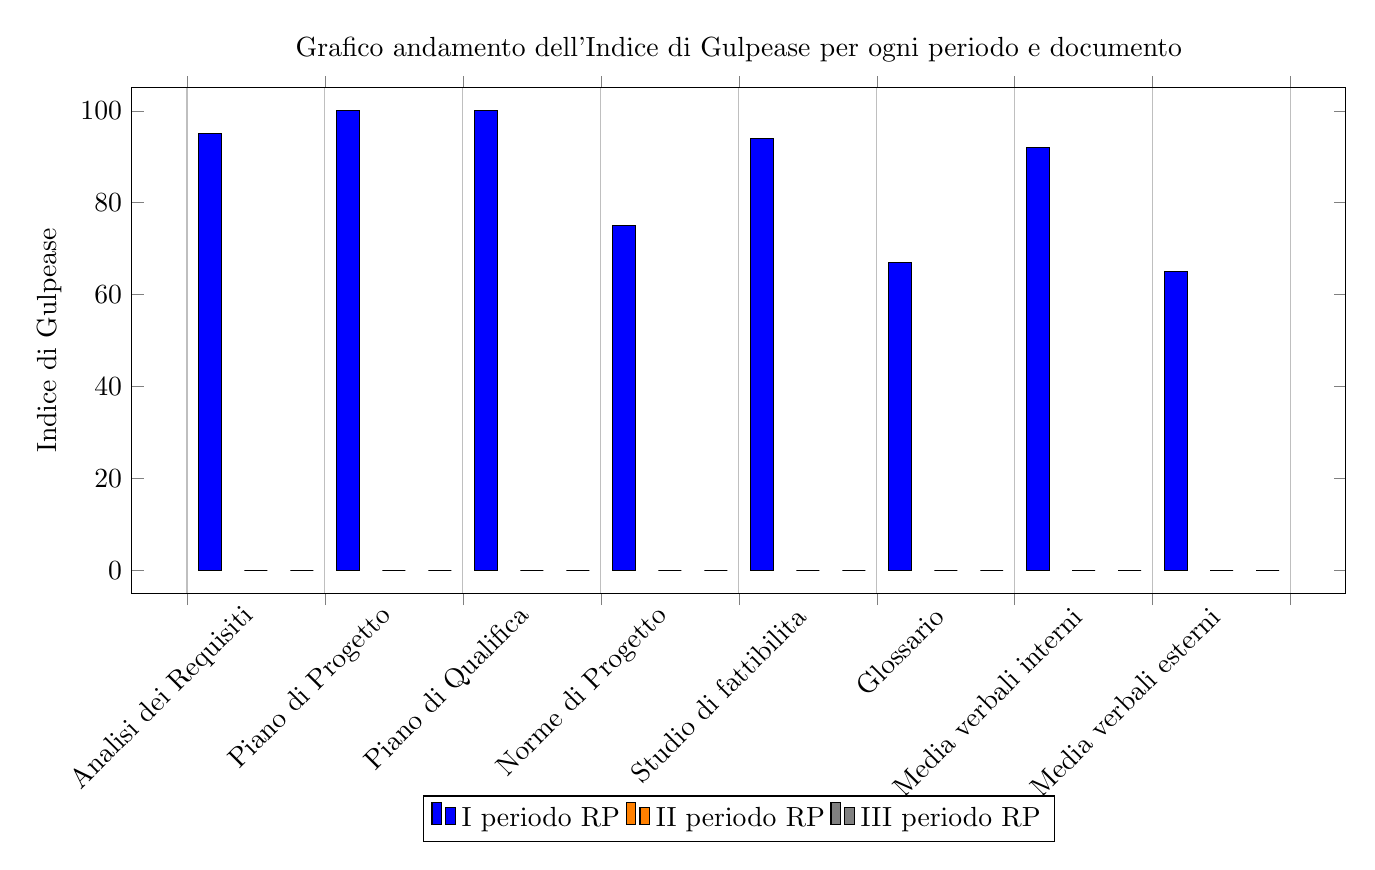
\begin{tikzpicture}

\begin{axis}[
title=Grafico andamento dell'Indice di Gulpease per ogni periodo e documento,
x tick label style={
	/pgf/number format/1000 sep=},
ylabel=Indice di Gulpease,
enlargelimits=0.05,
legend style={at={(0.5,-0.4)},
	anchor=north,legend columns=-1},
ybar interval=0.5,
symbolic x coords={Analisi dei Requisiti, Piano di Progetto, Piano di Qualifica, Norme di Progetto, Studio di fattibilita, Glossario,
	Media verbali interni, Media verbali esterni, tmp},%lasciare tmp come ultima colonna per poter visualizzare tutte le colonne tranne tmp
x tick label style={rotate=45,anchor=east},
xtick=data
]
\addplot[fill=blue] coordinates
{(Analisi dei Requisiti, 95) (Piano di Progetto, 100) (Piano di Qualifica, 100) 
	(Norme di Progetto, 75) (Studio di fattibilita, 94) (Glossario, 67)
	(Media verbali interni, 92) (Media verbali esterni, 65) (tmp, 100)};

\addplot [fill=orange] coordinates
{(Analisi dei Requisiti, 0) (Piano di Progetto, 0) (Piano di Qualifica, 0) 
	(Norme di Progetto, 0) (Studio di fattibilita, 0) (Glossario, 0)
	(Media verbali interni, 0) (Media verbali esterni, 0) (tmp, 0)};

\addplot [fill=gray] coordinates
{(Analisi dei Requisiti, 0) (Piano di Progetto, 0) (Piano di Qualifica, 0) 
	(Norme di Progetto, 0) (Studio di fattibilita, 0) (Glossario, 0) 
	(Media verbali interni, 0) (Media verbali esterni, 0) (tmp, 0)};

\legend{
	I periodo RP,
	II periodo RP,
	III periodo RP
}
\end{axis}
\end{tikzpicture}

\paragraph{MPC7 - Code coverage}

\paragraph{MPC8 - Schedule variance}
\pgfplotsset{width=17cm, height=8cm}
\begin{tikzpicture}

\begin{axis}[
title=Grafico andamento schedule variance per ogni periodo,
x tick label style={
	/pgf/number format/1000 sep=},
ylabel=SV,
enlargelimits=0.05,
legend style={at={(0.5,-0.4)},
	anchor=north,legend columns=-1},
ybar interval=0.33,
symbolic x coords={I periodo RP, II periodo RP, III periodo RP, tmp},%lasciare tmp come ultima colonna per poter visualizzare tutte le colonne tranne tmp
x tick label style={rotate=45,anchor=east},
xtick=data
]
\addplot[fill=blue] coordinates
{(I periodo RP, 0) (II periodo RP, 0) (III periodo RP, 0) (tmp, 100)};

\end{axis}
\end{tikzpicture}

\paragraph{MPC9 - Budget variance}
\pgfplotsset{width=17cm, height=8cm}
\begin{tikzpicture}

\begin{axis}[
title=Grafico andamento budget variance per ogni periodo,
x tick label style={
	/pgf/number format/1000 sep=},
ylabel=BV,
enlargelimits=0.05,
legend style={at={(0.5,-0.4)},
	anchor=north,legend columns=-1},
ybar interval=0.33,
symbolic x coords={I periodo RP, II periodo RP, III periodo RP, tmp},%lasciare tmp come ultima colonna per poter visualizzare tutte le colonne tranne tmp
x tick label style={rotate=45,anchor=east},
xtick=data
]
\addplot[fill=blue] coordinates
{(I periodo RP, 0) (II periodo RP, 0) (III periodo RP, 0) (tmp, 100)};

\end{axis}
\end{tikzpicture}


\paragraph{MPD1 - Attrattività della User Interface (UI)}
\pgfplotsset{width=17cm, height=8cm}
\rowcolors{2}{grigetto}{white}
\renewcommand{\arraystretch}{1.5}
\begin{longtable}{C{4cm} C{2cm} C{2cm} C{2cm} C{2cm}}
	\caption{Elenco delle valutazioni }\\
	\rowcolor{darkblue}
	\textcolor{white}{\textbf{Documento}} & \textcolor{white}{\textbf{I periodo RP}} &
	\textcolor{white}{\textbf{II periodo RP}} & \textcolor{white}{\textbf{III periodo RP}} \\
	\hline
	\endhead
	\textbf{Valutazione} & \textbf{-} & \textcolor{giallo}{\textbf{Attraente}} & \textcolor{giallo}{\textbf{Attraente}} \\
	
\end{longtable}

\paragraph{MPD2 - Complessità Ciclomatica del Software}
\pgfplotsset{width=17cm, height=8cm}
\begin{tikzpicture}

\begin{axis}[
title=Grafico andamento della complessità ciclomatica del software per ogni periodo,
x tick label style={
	/pgf/number format/1000 sep=},
ylabel=CCS,
enlargelimits=0.05,
legend style={at={(0.5,-0.4)},
	anchor=north,legend columns=-1},
ybar interval=0.33,
symbolic x coords={I periodo RP, II periodo RP, III periodo RP, tmp},%lasciare tmp come ultima colonna per poter visualizzare tutte le colonne tranne tmp
x tick label style={rotate=45,anchor=east},
xtick=data
]
\addplot[fill=blue] coordinates
{(I periodo RP, 0) (II periodo RP, 0) (III periodo RP, 0) (tmp, 100)};

\end{axis}
\end{tikzpicture}

\paragraph{MPD3 - Unità Documentate}
\pgfplotsset{width=17cm, height=8cm}
\begin{tikzpicture}

\begin{axis}[
title=Grafico percentuale dell'andamento del numero di unità documentate per ogni periodo,
x tick label style={
	/pgf/number format/1000 sep=},
ylabel=\% numero di unità documentate,
enlargelimits=0.05,
legend style={at={(0.5,-0.4)},
	anchor=north,legend columns=-1},
ybar interval=0.33,
symbolic x coords={I periodo RP, II periodo RP, III periodo RP, tmp},%lasciare tmp come ultima colonna per poter visualizzare tutte le colonne tranne tmp
x tick label style={rotate=45,anchor=east},
xtick=data
]
\addplot[fill=blue] coordinates
{(I periodo RP, 0) (II periodo RP, 0) (III periodo RP, 0) (tmp, 100)};

\end{axis}
\end{tikzpicture}

\paragraph{MPD6 - Maturità dei Test}

\paragraph{MPD7 - Profondità Strutturale dell'Interfaccia}
\pgfplotsset{width=17cm, height=8cm}
\begin{tikzpicture}

\begin{axis}[
title=Grafico dell'andamento del livello di profondità dell'interfaccia per ogni periodo,
x tick label style={
	/pgf/number format/1000 sep=},
ylabel=livello di profondità,
enlargelimits=0.05,
legend style={at={(0.5,-0.4)},
	anchor=north,legend columns=-1},
ybar interval=0.33,
symbolic x coords={I periodo RP, II periodo RP, III periodo RP, tmp},%lasciare tmp come ultima colonna per poter visualizzare tutte le colonne tranne tmp
x tick label style={rotate=45,anchor=east},
xtick=data
]
\addplot[fill=blue] coordinates
{(I periodo RP, 0) (II periodo RP, 0) (III periodo RP, 0) (tmp, 100)};

\end{axis}
\end{tikzpicture}
